\documentclass{beamer}
\usepackage{amsmath, amssymb}
\usepackage{graphicx}
\usepackage{listings}
\usepackage{color}

% Set up R code formatting
\definecolor{codegreen}{rgb}{0,0.6,0}
\definecolor{codegray}{rgb}{0.5,0.5,0.5}
\definecolor{codepurple}{rgb}{0.58,0,0.82}
\definecolor{backcolour}{rgb}{0.95,0.95,0.92}
\lstdefinestyle{Rstyle}{
    backgroundcolor=\color{backcolour},
    commentstyle=\color{codegreen},
    keywordstyle=\color{magenta},
    numberstyle=\tiny\color{codegray},
    stringstyle=\color{codepurple},
    basicstyle=\ttfamily\footnotesize,
    breakatwhitespace=false,
    breaklines=true,
    captionpos=b,
    keepspaces=true,
    numbers=left,
    numbersep=5pt,
    showspaces=false,
    showstringspaces=false,
    showtabs=false,
    tabsize=2
}

\title{Mixed Effects Models - Day 8}
\subtitle{Inference in Mixed Effects Models}
\author{Marieke Wesselkamp\\Department of Biometry and Environmental Systems Analysis\\Albert-Ludwigs-University of Freiburg (Germany)}
\date{February 2023}

\begin{document}

\frame{\titlepage}

\begin{frame}
    \frametitle{Hypothesis Testing}
    A procedure to control the type I error rate $\alpha$. It ensures that we incorrectly reject the null hypothesis (false positive) only with probability $\alpha$. There are four possible outcomes in hypothesis testing:
    
    \begin{table}[]
    \begin{tabular}{l|l|l}
    \textbf{} & \textbf{$H_0$ True} & \textbf{$H_0$ False} \\
    \hline
    No Rejection & Correct 95\% & Type II Error (20\%) \\
    Rejection & Type I Error (5\%) & Correct 80\%
    \end{tabular}
    \end{table}
\end{frame}

\begin{frame}
    \frametitle{p-value}
    The p-value is the probability of obtaining a result as extreme or more extreme than the observed data under the null hypothesis. It is not a guarantee that your alternative hypothesis is true.
    
    \begin{itemize}
        \item Small p-value $\Rightarrow$ unlikely data if $H_0$ is true.
        \item Large p-value does not mean $H_0$ is true; power may be low.
    \end{itemize}
    %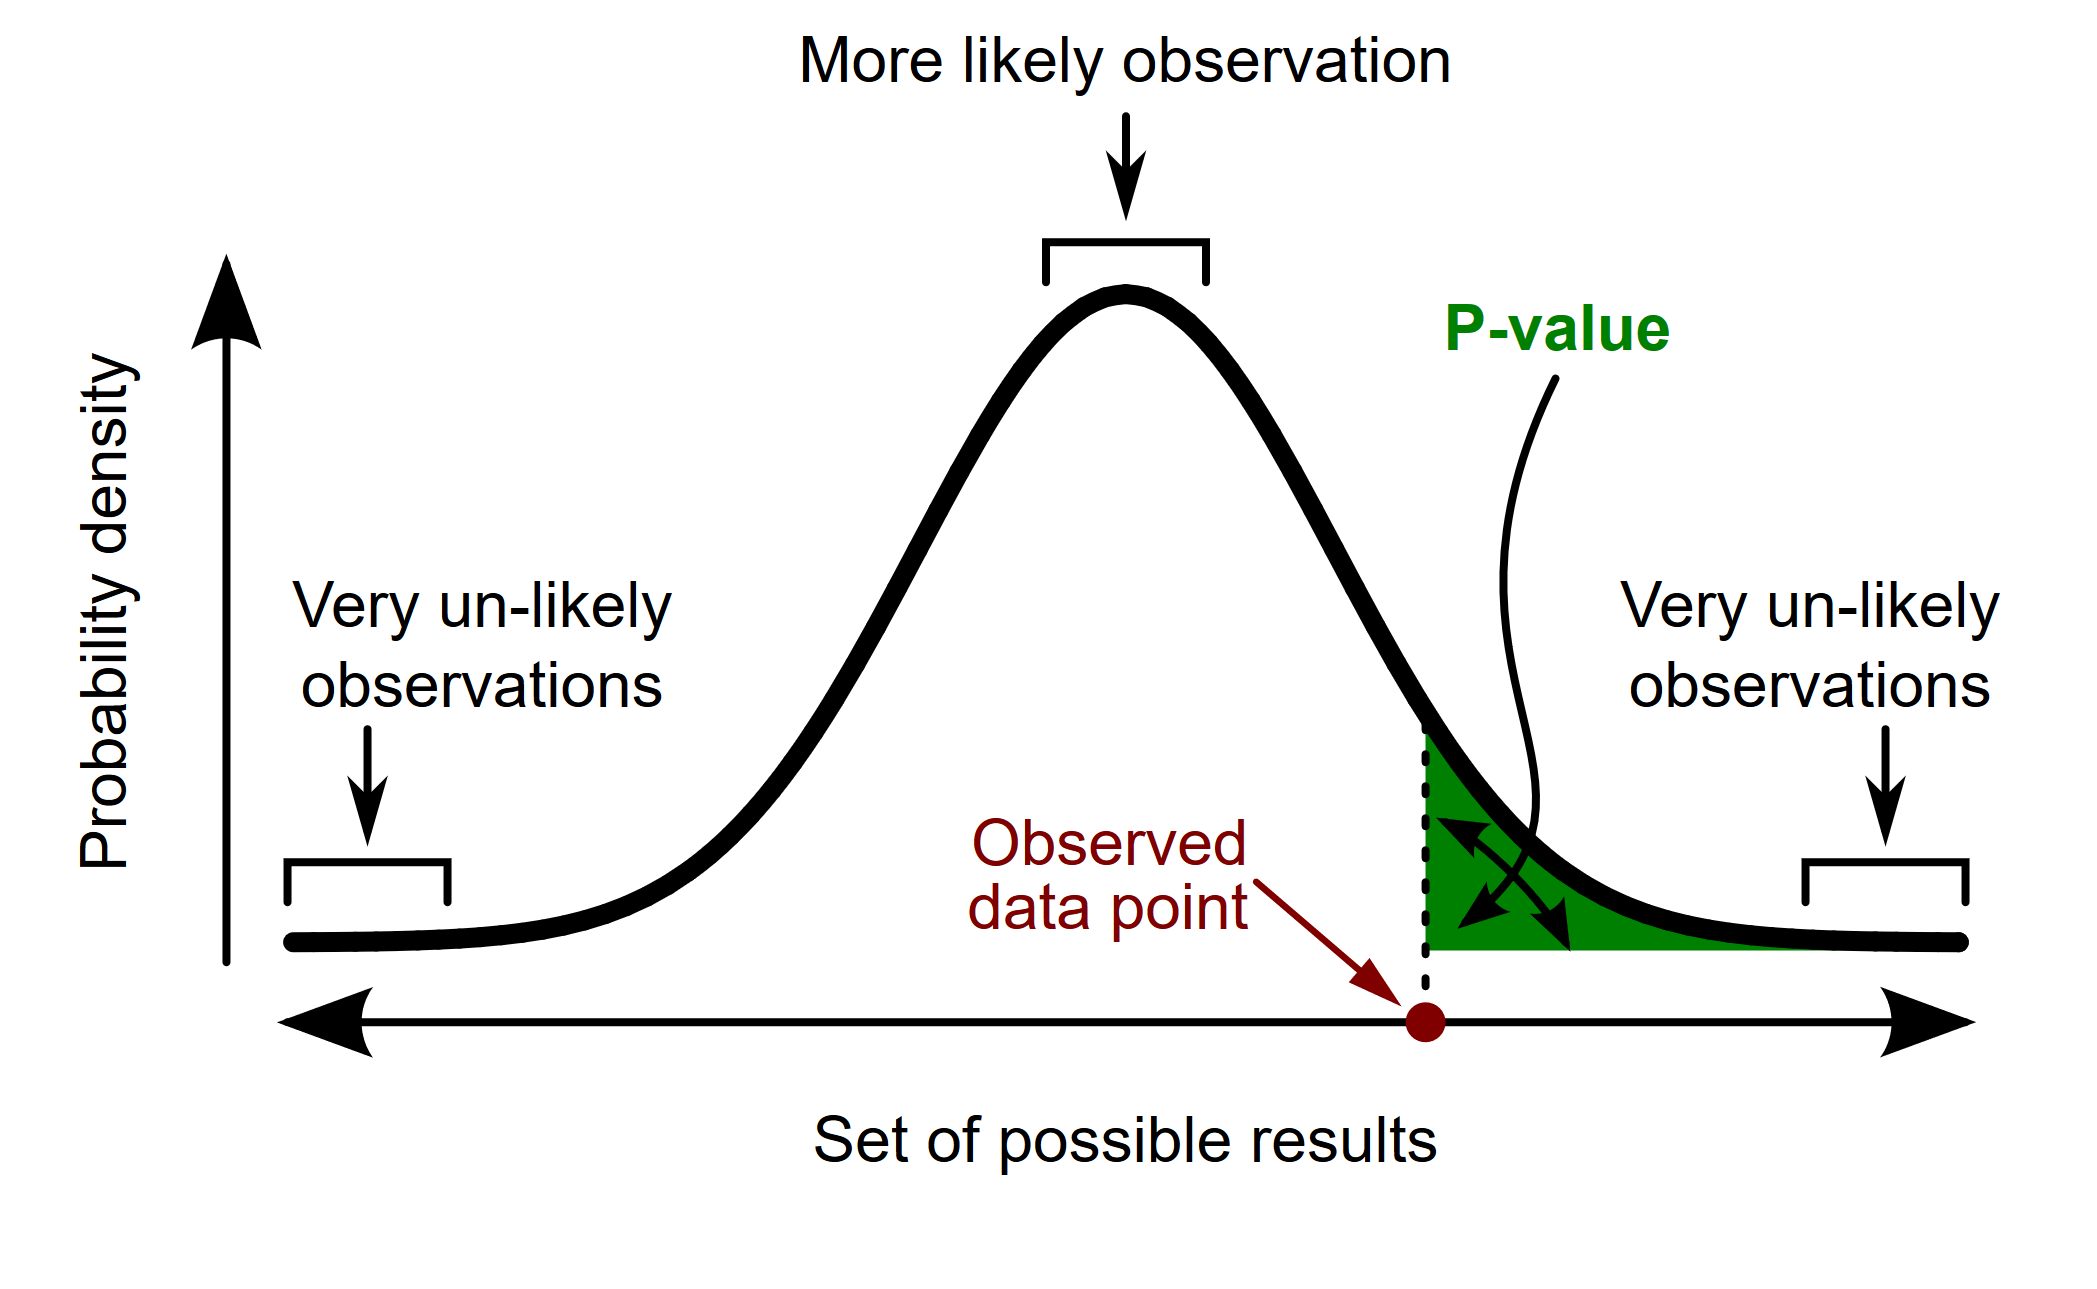
\includegraphics[width=0.6\textwidth]{p-value.png}
\end{frame}

\begin{frame}
    \frametitle{Steps of Hypothesis Testing}
    \begin{enumerate}
        \item Formulate a null hypothesis $H_0$
        \item Formulate an alternative hypothesis $H_A$
        \item Check assumptions
        \item Choose the appropriate test
        \item Calculate the test statistic
        \item Compare it to the null distribution
        \item Decide whether to reject $H_0$
    \end{enumerate}
\end{frame}

\begin{frame}
    \frametitle{Testing Parameters}
    In statistical modeling, hypothesis testing often involves testing whether parameters are zero:
    \[
    H_0: \beta = 0 \quad \text{vs.} \quad H_A: \beta \neq 0
    \]
\end{frame}

\begin{frame}
    \frametitle{Issues with Hypothesis Testing}
    \begin{itemize}
        \item Black-or-white, yes-or-no decisions.
        \item Often overlooks effect size, parameter estimation, and uncertainty.
        \item Emphasizes falsification.
    \end{itemize}
    Keep it simple: test one question per dataset.
\end{frame}

\begin{frame}
    \frametitle{Single Parameter Test}
    Consider the model:
    \[
    size_{ij} = \beta_0 + \beta_1 \cdot food + \beta_2 \cdot food^2 + \epsilon_{ij}
    \]
    Testing whether the quadratic term $\beta_2 = 0$. This can be done via t-tests in a model summary.
\end{frame}

\begin{frame}
    \frametitle{Group Parameter Test}
    Testing whether both $\beta_1 = 0$ and $\beta_2 = 0$. This can be done using an F-test in ANOVA.
\end{frame}

\begin{frame}
    \frametitle{Testing in Mixed Effects Models}
    In Mixed Effects Models, you can test:
    \begin{itemize}
        \item Variance components (random effects).
        \item Fixed effects.
    \end{itemize}
\end{frame}

\begin{frame}
    \frametitle{Variance Components}
    Questions to test:
    \begin{itemize}
        \item Is there a correlation between a random slope and random intercept?
        \item Is there a random slope or random intercept?
    \end{itemize}
\end{frame}

\begin{frame}
    \frametitle{General Advice on Random Effects Testing}
    Keep the random effects structure maximal instead of deciding on random components based on p-values.
\end{frame}

\begin{frame}
    \frametitle{Testing with REML}
    Random intercept vs random slope:
    \[
    \mathbf{G} = \begin{pmatrix}
    var_{11} & covar_{12} \\
    covar_{21} & var_{22}
    \end{pmatrix}
    \]
    Test whether the covariance or variance components are zero.
\end{frame}

\begin{frame}
    \frametitle{Testing Methods}
    \begin{itemize}
        \item Likelihood Ratio Test (LRT)
        \item Parametric Bootstrapping
    \end{itemize}
\end{frame}

\begin{frame}
    \frametitle{Log-Likelihood Ratio Test (LRT)}
    Compares two nested models (one more complex, one simpler) using the difference in their log-likelihoods. The result is approximately $\chi^2$ distributed. However, this approximation breaks down when testing at the boundary (e.g., variances cannot be negative).
\end{frame}

\begin{frame}
    \frametitle{Parametric Bootstrapping}
    Model comparison technique for nested models:
    \begin{itemize}
        \item Simulate data under both models.
        \item Fit the models to the simulated data.
        \item Calculate LRT values and obtain the p-value from the distribution of these values.
    \end{itemize}
\end{frame}

\begin{frame}
    \frametitle{Testing Fixed Effects}
    Common questions:
    \begin{itemize}
        \item Is there a linear or nonlinear trend?
        \item Is a variable causing the response?
        \item Is an interaction relevant?
    \end{itemize}
\end{frame}

\begin{frame}
    \frametitle{Multiple Testing Warning}
    Avoid multiple testing; test one question per dataset.
\end{frame}

\begin{frame}
    \frametitle{Model Selection with Information Criteria}
    For non-nested models, use an Information Criterion:
    \[
    AIC_c = -2 \ell + 2 p + \frac{2p(p+1)}{n-p-1}
    \]
    where $\ell$ is the log-likelihood, $p$ is the number of parameters, and $n$ is the sample size.
\end{frame}

\begin{frame}
    \frametitle{Bayesian Information Criterion (BIC)}
    An alternative to AIC:
    \[
    BIC = -2 \ell + p \cdot \log(n)
    \]
    Smaller values indicate better models.
\end{frame}

\begin{frame}
    \frametitle{Explained Variance ($R^2$)}
    The proportion of total variance explained by a model:
    \[
    R^2 = \frac{Var_{Effect}}{Var_{Total}} \times 100
    \]
    In Mixed Effects Models, we distinguish between:
    \begin{itemize}
        \item Marginal $R^2$: Fixed effects only.
        \item Conditional $R^2$: Fixed and random effects.
    \end{itemize}
\end{frame}

\begin{frame}
    \frametitle{Using R to Calculate $R^2$}
    \lstset{style=Rstyle}
    \begin{lstlisting}
    library(lme4)
    library(MuMIn)
    mod <- lmer(distance ~ age*Sex + (age | Subject), data = Orthodont)
    r.squaredGLMM(mod)
    \end{lstlisting}
\end{frame}

\begin{frame}
    \frametitle{Intraclass Correlation Coefficient (ICC)}
    ICC quantifies the proportion of total variance attributable to group differences:
    \[
    \text{ICC} = \frac{\sigma^2_{group}}{\sigma^2_{group} + \sigma^2_{residual}}
    \]
\end{frame}

% \begin{frame}[fragile]
%     \frametitle{Calculate ICC in R}
%     \lstset{style=Rstyle}
%     \begin{lstlisting}
%     mod <- lmer(distance ~ age*Sex + (age | Subject), data = Orthodont)
%     icc(mod)
%     \end{lstlisting}
% \end{frame}

\begin{frame}
    \frametitle{ICC for Random Intercept Model}
    ICC for random intercept models equals the variance partitioning coefficient:
    \[
    \text{ICC} = \frac{\sigma^2_{intercept}}{\sigma^2_{intercept} + \sigma^2_{residual}}
    \]
\end{frame}

\begin{frame}
    \frametitle{Convenience Packages in R}
    Useful packages:
    \begin{itemize}
        \item For summary stats: `performance`, `MuMIn`, `afex`.
        \item For ICC: `performance`.
        \item For model comparison: `lmerTest`.
        \item For plotting: `performance`, `interplot`.
    \end{itemize}
\end{frame}

\begin{frame}
    \frametitle{Recapitulation Day 9}
    Topics covered today:
    \begin{itemize}
        \item Hypothesis testing: single vs. multiple parameter tests.
        \item Testing variance components and fixed effects.
        \item When to use REML or ML.
    \end{itemize}
\end{frame}

\end{document}